
\section{Motivation}

\begin{frame}{Trees and Pattern Matching}
\begin{minipage}{.5\textwidth}

\newcommand{\mknode}[3]{\draw (#1,#2)  circle (.27cm) node[align=center] {\IdrisData{#3}};}
\newcommand{\mkleaf}[2]{\draw[fill=black] (#1,#2) node[align=center] {} +(-.1cm,-.1cm) rectangle +(.1cm,.1cm);}

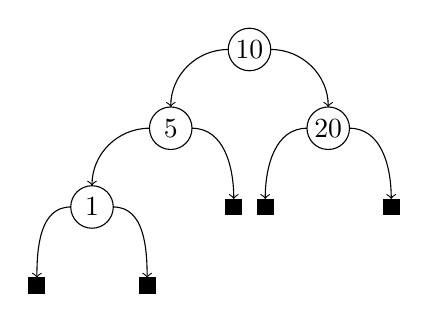
\begin{tikzpicture}
\mknode{0}{0}{10}
  \mknode{-1}{-1}{5};
    \mknode{-2}{-2}{1};
      \mkleaf{-2.7}{-3};
      \mkleaf{-1.3}{-3};
  \mkleaf{-.2}{-2}
  \mknode{1}{-1}{20}
    \mkleaf{.2}{-2}
    \mkleaf{1.8}{-2}

\draw [->] (-0.27,0) to [out=180,in=90] (-1,-.73);
  \draw [->] (-1.27,-1) to [out=180,in=90] (-2,-1.73);
    \draw [->] (-2.27,-2) to [out=180,in=90] (-2.7,-2.9);
    \draw [->] (-1.73,-2) to [out=0,in=90] (-1.3,-2.9);
  \draw [->] (-.73,-1) to [out=0,in=90] (-.2,-1.9);
\draw [->] (0.27,0) to [out=0,in=90] (1,-.73);
  \draw [->] (.73,-1) to [out=180,in=90] (.2,-1.9);
  \draw [->] (1.27,-1) to [out=0,in=90] (1.8,-1.9);
\end{tikzpicture}

\end{minipage}\hfill
\begin{minipage}{.45\textwidth}
  \ExecuteMetaData[Motivating.idr.tex]{motivation}
\end{minipage}
\end{frame}

\begin{frame}[fragile]{Serialised Data and Pointer Manipulations}
\begin{hexdump}
01 01 01 00 \hexadata{01} 00 \hexadata{05} 00 \hexadata{0a} 01 00 \hexadata{14} 00
\end{hexdump}
\begin{overlayarea}{\linewidth}{6cm}
\begin{onlyenv}<2->
\begin{lstlisting}
int sumAt (int buf[], int *ptr, int *acc) {
  int tag = buf[*ptr]; (*ptr)++;
  switch (tag) {
    case 0: return 0;
    case 1:
      sumAt(buf, ptr, acc);
      int val = buf[*ptr]; (*ptr)++;
      *acc += val;
      sumAt(buf, ptr, acc);
      return 0;
    default: exit(-1); }}
\end{lstlisting}

\end{onlyenv}
\end{overlayarea}
\end{frame}

\begin{frame}{Seamless}

  \vspace*{2em}

  \begin{minipage}{.6\textwidth}
    \ExecuteMetaData[SaferIndexed.idr.tex]{tsum}
  \end{minipage}\hfill

  \hfill\begin{minipage}{.6\textwidth}
    \ExecuteMetaData[SaferIndexed.idr.tex]{rsum}
  \end{minipage}
\end{frame}


\begin{frame}{Correct}
  \ExecuteMetaData[Data/Singleton.idr.tex]{singleton}
  \vfill
  \ExecuteMetaData[SaferIndexed.idr.tex]{csum}
\end{frame}


\begin{frame}{Generic}
  %% \ExecuteMetaData[Serialised/Desc.idr.tex]{data}

  %% \vspace*{2em}

  %% \ExecuteMetaData[SaferIndexed.idr.tex]{viewfun}

  %% \vspace*{2em}

  \ExecuteMetaData[SaferIndexed.idr.tex]{foldtype}
\end{frame}
